% Copyright 2021 Wuping Xin

% This program is free software: you can redistribute it and/or modify it under
% the terms of the GNU General Public License as published by the Free Software
% Foundation, either version 3 of the License, or (at your option) any later
% version.

% This program is distributed in the hope that it will be useful,but WITHOUT ANY
% WARRANTY; without even the implied warranty of MERCHANTABILITY or FITNESS FOR A
% PARTICULAR PURPOSE. See the GNU General Public License for more details. You
% should have received a copy of the GNU General Public License along with this
% program. If not, see <http://www.gnu.org/licenses/>.

% This template is based on IEEE/ISO/IEC 29148-2018, Section 9.6.

\documentclass{scrreprt}

\usepackage[brazil]{babel}
\usepackage{booktabs}
\usepackage{caption}
\usepackage{geometry}
\usepackage{graphicx}
\usepackage{hyperref}
\usepackage[utf8]{inputenc}
\usepackage{pdflscape}
\usepackage{tikz}
\usepackage{underscore}
\usepackage[table,xcdraw]{xcolor}

\usetikzlibrary{arrows.meta,backgrounds,fit,positioning,shapes.geometric}

\def\myauthorname{Bryan Alvarenga -- 272426 \\
	Igor Bassetto Menon -- 274582 \\
	Juan Pedrozo -- 273889 \\
	Kauã Gustavo da Fonseca Rodrigues -- 273722 \\
	Rafael Dias Garcia -- 272207 \\
	Vitor Yago Ferreira dos Santos -- 272261}

\def\mykeywords{ERS, GeekHub, marketplace, requisitos de software}
\def\myorganization{GuildCode\\UNIFIO\\Ourinhos, Brasil}
\def\myreviewer{Thiago Henrique Pereira Paiva}
\def\mysubject{GeekHub}
\def\mytitle{Especificação de Requisitos de Software}
\def\myversion{1.0}

\setcounter{tocdepth}{1}

\newenvironment{fieldlist}
	{\renewcommand{\labelitemi}{--}\begin{itemize}}
	{\end{itemize}}

\hypersetup{
	pdftitle={\mytitle},          % title
	pdfauthor={Grupo GuildCode},  % author
	pdfsubject={\mysubject},      % subject of the document
	pdfkeywords={\mykeywords},    % list of keywords
	colorlinks=true,              % false: boxed links; true: colored links
	linkcolor=blue,               % color of internal links
	citecolor=black,              % color of links to bibliography
	filecolor=black,              % color of file links
	urlcolor=purple,              % color of external links
	linktoc=page                  % only page is linked
}

\begin{document}
\thispagestyle{empty}

\begin{flushright}
    \rule{\textwidth}{5pt}\vskip 0.8cm
    \begin{bfseries}
        \LARGE{Especificação de Requisitos de Software}\\
        \vspace{0.8cm}
        para o \\
        \vspace{0.8cm}
        \Huge{\mysubject}\\
        \vspace{1.9cm}
        \Large{Versão \myversion}\\
    \end{bfseries}
        \vfill
        \large 	Preparado por\\
        \vspace{0.25cm}
        \LARGE \textbf{\myauthorname}
        \vfill
        \large 	Revisado por\\
        \vspace{0.25cm}
        \LARGE \textbf{\myreviewer}
        \vfill
        \large \myorganization\\
        \vspace{0.5cm}
	    \today\\
\end{flushright}

\chapter*{Histórico de Revisões}
\setcounter{page}{1}
\begin{center}
	\begin{tabular}{@{} p{3cm} l p{5.4cm} l @{}}
		\toprule
		\textbf{Nome}           & \textbf{Data} & \textbf{Motivo da mudança} & \textbf{Versão} \\
		\midrule
		Grupo GuildCode         & \today        & Versão inicial             & 1.0             \\
		\bottomrule
	\end{tabular}
\end{center}

\tableofcontents

\chapter{Introdução}

\section{Propósito}

Este documento define os requisitos do sistema GeekHub. O GeekHub será um
marketplace para a compra e venda de itens geek e colecionáveis.

O documento define:
\begin{fieldlist}
	\item funções de sistema;
	\item perfis de usuário;
	\item regras de negócio;
	\item requisitos não funcionais;
	\item limites do MVP.
\end{fieldlist}

\section{Escopo}

O GeekHub deve conectar compradores e vendedores de itens geek e colecionáveis.
A plataforma deve permitir o anúncio, a pesquisa e a compra de produtos.

O MVP deve incluir:
\begin{fieldlist}
	\item cadastro de usuários;
	\item edição de perfil;
	\item autenticação;
	\item gerenciamento de anúncios;
	\item pesquisa de produtos;
	\item filtros;
	\item carrinho;
	\item pedidos;
	\item avaliações;
	\item administração.
\end{fieldlist}

\section{Definições}

\begin{center}
	\begin{tabular}{@{} l p{10.5cm} @{}}
		\toprule
		\textbf{Termo}         & \textbf{Definição}                                              \\
		\midrule
		RF                     & Requisito funcional                                             \\
		RNF                    & Requisito não funcional                                         \\
		RN                     & Regra de negócio                                                \\
		Usuário                & Pessoa que possui uma conta no sistema                          \\
		Usuário Comum          & Usuário que pode comprar e vender produtos e gerenciar os próprios anúncios \\
		Administrador          & Usuário responsável pela administração da plataforma            \\
		Produto                & Item disponibilizado para venda                                 \\
		Anúncio                & Registro que disponibiliza um produto no marketplace            \\
		Pedido                 & Registro de uma compra                                          \\
		Critério de verificação & Condição objetiva utilizada para verificar o atendimento de um requisito \\
		ERS                    & Especificação de Requisitos de Software                         \\
		MVP                    & Primeira versão utilizável do sistema                           \\
		LGPD                   & Lei Geral de Proteção de Dados Pessoais                         \\
		\bottomrule
	\end{tabular}
\end{center}

\chapter{Descrição Geral}

\section{Perspectiva do produto}

A compra e a venda de itens geek hoje acontecem em marketplaces genéricos, redes
sociais e grupos de mensagens. Essa fragmentação aumenta o tempo de busca, reduz a
padronização das informações e dificulta que vendedores encontrem um público
interessado. Para colecionáveis, diferenças de edição, fabricante e conservação
tornam a busca genérica ainda menos eficiente.

\section{Perfis de usuário}

\begin{center}
	\begin{tabular}{@{} l p{4cm} p{6.5cm} @{}}
		\toprule
		\textbf{Perfil}   & \textbf{Objetivos}                      & \textbf{Necessidades}                                                                                                                                 \\
		\midrule
		Usuário Comum     & Comprar e vender itens geek e colecionáveis. & Pesquisar produtos, visualizar anúncios, realizar compras, cadastrar produtos para venda, gerenciar anúncios e acompanhar pedidos. \\
		Administrador     & Administrar a plataforma.                & Gerenciar usuários, anúncios e categorias, além de remover conteúdos que violem as regras do marketplace.                                          \\
		\bottomrule
	\end{tabular}
\end{center}

\section{Diagrama de casos de uso}

A figura a seguir apresenta o diagrama de casos de uso do sistema, com os
perfis de usuário e as funcionalidades descritas nas próximas seções.

\clearpage
\begin{figure}[htbp]
    \centering
    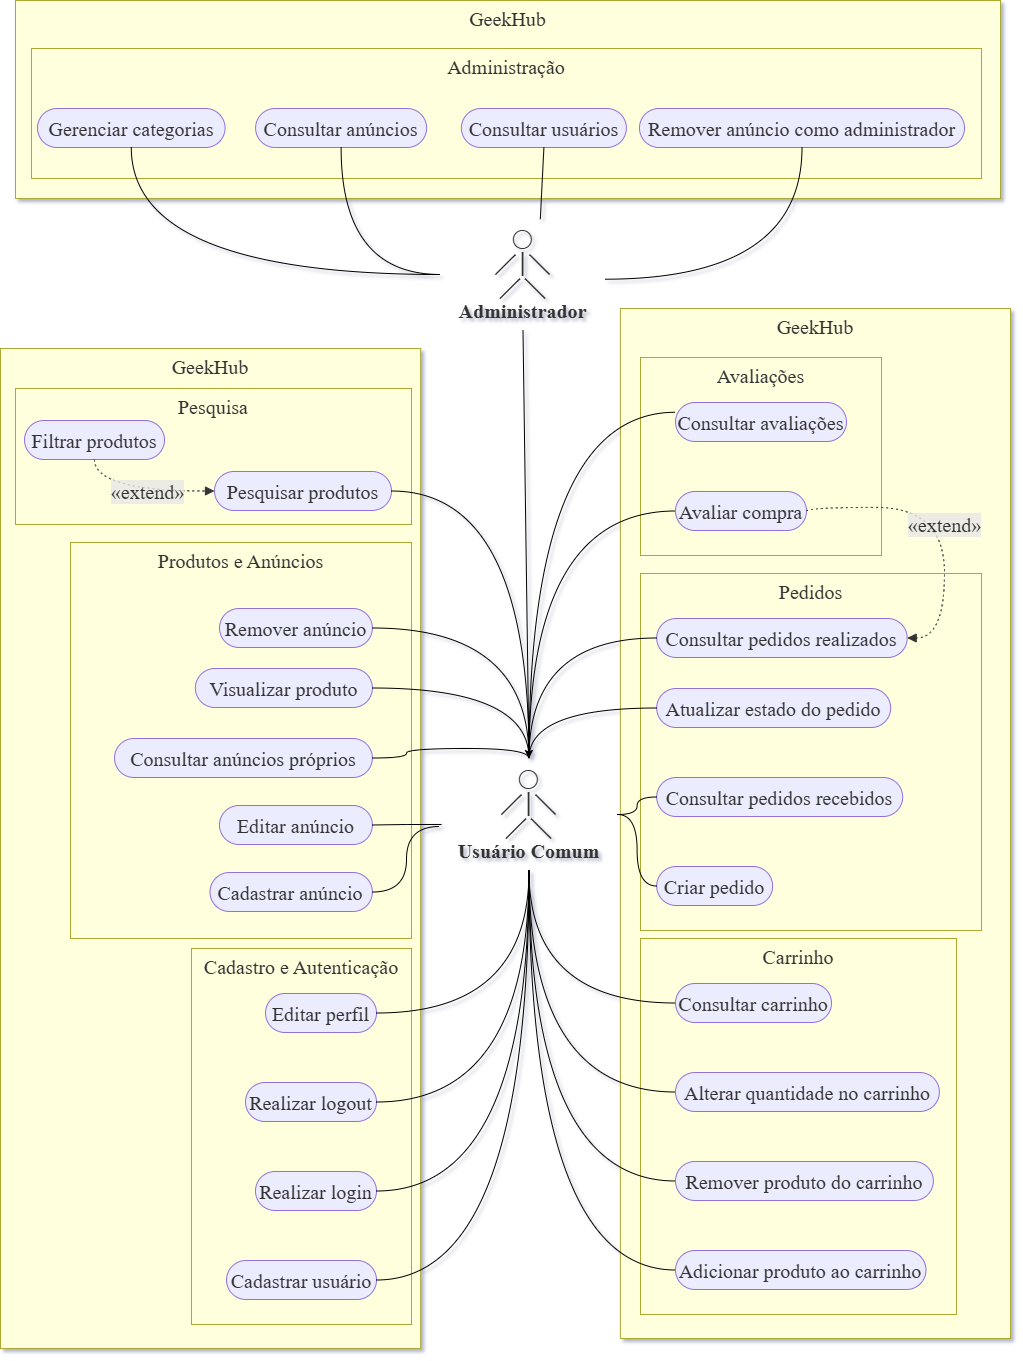
\includegraphics[height=0.88\textheight]{imagens/geekhub.drawio.png}
    \caption{Diagrama de casos de uso do sistema GeekHub.}
    \label{fig:casos-de-uso-geekhub}
\end{figure}
\clearpage

\section{Suposições}

\begin{center}
	\begin{tabular}{@{} l p{11.5cm} @{}}
		\toprule
		\textbf{Tipo}          & \textbf{Suposição}                                                                 \\
		\midrule
		Usuário                & Um usuário comum pode comprar e vender produtos.                                    \\
		Acesso                 & O usuário deve possuir uma conta para comprar ou vender.                             \\
		Permissão              & O administrador possui permissões diferentes do usuário comum.                       \\
		Pagamento              & O MVP não terá pagamento integrado.                                                  \\
		Frete                  & O MVP não terá cálculo automático de frete.                                          \\
		Comunicação            & O MVP não terá chat entre usuários.                                                  \\
		Troca                  & O MVP não terá sistema de troca de produtos.                                         \\
		Plataforma             & O sistema será utilizado por meio de uma aplicação web.                              \\
		\bottomrule
	\end{tabular}
\end{center}

\chapter{Requisitos Específicos}

\section{Cadastro e autenticação}

\subsection{RF01 -- Cadastrar usuário}
O sistema deve permitir o cadastro de um usuário.
\begin{itemize}
	\item \textbf{RN01} -- O e-mail informado deve ser único;
	\item \textbf{RN02} -- O usuário deve preencher todos os campos obrigatórios;
	\item \textbf{RN03} -- O usuário deve informar um e-mail válido.
\end{itemize}

\subsection{RF02 -- Realizar login}
O sistema deve permitir que um usuário cadastrado realize login.
\begin{itemize}
	\item \textbf{RN04} -- O usuário deve possuir uma conta cadastrada;
	\item \textbf{RN05} -- As credenciais informadas devem ser válidas.
\end{itemize}

\subsection{RF03 -- Realizar logout}
O sistema deve permitir que um usuário autenticado encerre sua sessão.

\subsection{RF04 -- Editar perfil}
O sistema deve permitir que o usuário altere os dados permitidos do próprio perfil.
\begin{itemize}
	\item \textbf{RN06} -- O usuário somente pode editar o próprio perfil;
	\item \textbf{RN07} -- O novo e-mail não pode estar associado a outro usuário.
\end{itemize}

\section{Produtos e anúncios}

\subsection{RF05 -- Cadastrar anúncio}
O sistema deve permitir que o usuário cadastre um anúncio.

O anúncio deve possuir:
\begin{fieldlist}
	\item nome;
	\item descrição;
	\item categoria;
	\item preço;
	\item quantidade;
	\item estado de conservação;
	\item condição do produto;
	\item imagem.
\end{fieldlist}

\begin{itemize}
	\item \textbf{RN08} -- Todo anúncio deve estar associado ao usuário que o cadastrou;
	\item \textbf{RN09} -- O preço deve ser maior que zero;
	\item \textbf{RN10} -- A quantidade disponível deve ser maior que zero;
	\item \textbf{RN11} -- O anúncio deve pertencer a uma categoria ativa;
	\item \textbf{RN12} -- O anúncio deve possuir pelo menos uma imagem.
\end{itemize}

\subsection{RF06 -- Editar anúncio}
O sistema deve permitir que o usuário edite um anúncio.
\begin{itemize}
	\item \textbf{RN13} -- Somente o responsável pelo anúncio pode editar o anúncio;
	\item \textbf{RN14} -- O preço deve permanecer maior que zero;
	\item \textbf{RN15} -- O anúncio deve permanecer associado a uma categoria ativa.
\end{itemize}

\subsection{RF07 -- Remover anúncio}
O sistema deve permitir que o usuário remova um anúncio.
\begin{itemize}
	\item \textbf{RN16} -- Somente o responsável pelo anúncio ou um administrador pode remover o anúncio.
\end{itemize}

\subsection{RF08 -- Consultar anúncios próprios}
O sistema deve permitir que o usuário consulte os anúncios cadastrados por ele.
\begin{itemize}
	\item \textbf{RN17} -- O usuário deve estar autenticado para consultar seus anúncios.
\end{itemize}

\subsection{RF09 -- Visualizar produto}
O sistema deve permitir que o usuário visualize os dados públicos de um produto.

O sistema deve mostrar:
\begin{fieldlist}
	\item nome;
	\item imagens;
	\item descrição;
	\item categoria;
	\item preço;
	\item estado de conservação;
	\item condição;
	\item quantidade disponível;
	\item informações públicas do usuário responsável pelo anúncio.
\end{fieldlist}

\begin{itemize}
	\item \textbf{RN18} -- Somente anúncios disponíveis devem permitir a realização de uma compra.
\end{itemize}

\section{Pesquisa}

\subsection{RF10 -- Pesquisar produtos}
O sistema deve permitir a pesquisa de produtos pelo nome.
\begin{itemize}
	\item \textbf{RN19} -- A pesquisa deve apresentar somente anúncios disponíveis para compra.
\end{itemize}

\subsection{RF11 -- Filtrar produtos}
O sistema deve permitir o uso de filtros durante a pesquisa.

O sistema deve mostrar:
\begin{fieldlist}
	\item categoria;
	\item faixa de preço;
	\item estado de conservação;
	\item produto novo ou usado.
\end{fieldlist}

\begin{itemize}
	\item \textbf{RN20} -- O sistema deve aplicar todos os filtros selecionados pelo usuário.
\end{itemize}

\section{Carrinho}

\subsection{RF12 -- Adicionar produto ao carrinho}
O sistema deve permitir que o usuário comum adicione um produto ao carrinho.
\begin{itemize}
	\item \textbf{RN21} -- O produto deve possuir quantidade disponível;
	\item \textbf{RN22} -- A quantidade adicionada não pode ser maior que a quantidade disponível.
\end{itemize}

\subsection{RF13 -- Remover produto do carrinho}
O sistema deve permitir que o usuário comum remova um produto do carrinho.

\subsection{RF14 -- Alterar quantidade do produto no carrinho}
O sistema deve permitir que o usuário comum altere a quantidade de um produto no carrinho.
\begin{itemize}
	\item \textbf{RN23} -- A quantidade deve ser maior que zero;
	\item \textbf{RN24} -- A quantidade não pode ser maior que o estoque disponível.
\end{itemize}

\subsection{RF15 -- Consultar carrinho}
O sistema deve permitir que o usuário comum consulte o carrinho.

O sistema deve mostrar:
\begin{fieldlist}
	\item produtos;
	\item quantidades;
	\item preço de cada produto;
	\item valor total.
\end{fieldlist}

\begin{itemize}
	\item \textbf{RN25} -- O valor total deve considerar todos os produtos e suas respectivas quantidades.
\end{itemize}

\section{Pedidos}

\subsection{RF16 -- Criar pedido}
O sistema deve permitir que o usuário comum crie um pedido com os produtos do carrinho.
\begin{itemize}
	\item \textbf{RN26} -- O carrinho deve possuir pelo menos um produto;
	\item \textbf{RN27} -- Todos os produtos devem possuir quantidade disponível;
	\item \textbf{RN28} -- A quantidade solicitada não pode ser maior que a quantidade disponível.
\end{itemize}

\subsection{RF17 -- Consultar pedidos realizados}
O sistema deve permitir que o usuário comum consulte seus pedidos.
\begin{itemize}
	\item \textbf{RN29} -- O usuário comum somente pode consultar pedidos associados à sua conta.
\end{itemize}

\subsection{RF18 -- Consultar pedidos recebidos}
O sistema deve permitir que o usuário comum consulte os pedidos que contenham produtos anunciados por ele.
\begin{itemize}
	\item \textbf{RN30} -- O usuário comum somente pode consultar pedidos relacionados aos seus anúncios.
\end{itemize}

\subsection{RF19 -- Atualizar estado do pedido}
O sistema deve permitir a atualização do estado do pedido.

Os estados são:
\begin{fieldlist}
	\item Criado;
	\item Confirmado;
	\item Enviado;
	\item Concluído;
	\item Cancelado.
\end{fieldlist}

\begin{itemize}
	\item \textbf{RN31} -- Um pedido deve possuir somente um estado por vez;
	\item \textbf{RN32} -- O estado informado deve ser um dos estados definidos pelo sistema.
\end{itemize}

\section{Avaliações}

\subsection{RF20 -- Avaliar compra}
O sistema deve permitir que o usuário comum avalie uma compra.

A avaliação deve possuir:
\begin{fieldlist}
	\item nota de 1 a 5;
	\item comentário opcional.
\end{fieldlist}

\begin{itemize}
	\item \textbf{RN33} -- Somente uma compra concluída pode ser avaliada;
	\item \textbf{RN34} -- Somente o usuário comum responsável pelo pedido pode criar a avaliação;
	\item \textbf{RN35} -- Cada compra pode possuir somente uma avaliação;
	\item \textbf{RN36} -- A nota deve possuir um valor entre 1 e 5.
\end{itemize}

\subsection{RF21 -- Consultar avaliações}
O sistema deve permitir que os usuários consultem as avaliações públicas de outro usuário.
\begin{itemize}
	\item \textbf{RN37} -- Somente avaliações registradas devem fazer parte da nota pública do usuário.
\end{itemize}

\section{Administração}

\subsection{RF22 -- Consultar usuários}
O sistema deve permitir que o administrador consulte os usuários cadastrados.
\begin{itemize}
	\item \textbf{RN38} -- Somente um administrador pode acessar a função de consulta administrativa de usuários.
\end{itemize}

\subsection{RF23 -- Consultar anúncios}
O sistema deve permitir que o administrador consulte os anúncios cadastrados.
\begin{itemize}
	\item \textbf{RN39} -- Somente um administrador pode acessar a consulta administrativa de anúncios.
\end{itemize}

\subsection{RF24 -- Remover anúncio como administrador}
O sistema deve permitir que o administrador remova um anúncio.
\begin{itemize}
	\item \textbf{RN40} -- O administrador pode remover anúncios que violem as regras da plataforma.
\end{itemize}

\subsection{RF25 -- Gerenciar categorias}
O sistema deve permitir que o administrador:
\begin{fieldlist}
	\item cadastre categorias;
	\item edite categorias;
	\item desative categorias.
\end{fieldlist}

\begin{itemize}
	\item \textbf{RN41} -- Somente um administrador pode gerenciar categorias;
	\item \textbf{RN42} -- Uma categoria desativada não pode ser usada em novos anúncios.
\end{itemize}

\section{Requisitos Não Funcionais}

Cada requisito não funcional é acompanhado de critérios de verificação que
permitem avaliar objetivamente o seu atendimento.

\subsection{RNF01 -- Desempenho}
O sistema deve responder a 95\% das operações de consulta em até 2 segundos no
ambiente definido para os testes.

Critério de verificação:
\begin{fieldlist}
	\item O tempo deve ser medido entre a solicitação do usuário e o recebimento da resposta do sistema.
\end{fieldlist}

\subsection{RNF02 -- Segurança da comunicação}
O sistema deve transmitir dados pessoais, credenciais e dados de sessão somente
por meio de comunicação criptografada (HTTPS) entre o usuário e a plataforma.

Critério de verificação:
\begin{fieldlist}
	\item Nenhum dado pessoal, credencial ou dado de sessão deve ser transmitido em formato não criptografado.
\end{fieldlist}

\subsection{RNF03 -- Proteção de credenciais}
O sistema deve proteger as credenciais dos usuários.

Critérios de verificação:
\begin{fieldlist}
	\item A senha do usuário não deve ser exibida em texto legível;
	\item A senha do usuário não deve ser armazenada em formato diretamente legível.
\end{fieldlist}

\subsection{RNF04 -- Controle de acesso}
O sistema deve permitir que cada usuário execute somente as operações
compatíveis com o seu perfil (usuário comum ou administrador).

Critérios de verificação:
\begin{fieldlist}
	\item Somente o administrador pode executar funções administrativas;
	\item Um usuário não pode alterar dados privados de outro usuário.
\end{fieldlist}

\subsection{RNF05 -- Responsividade}
O sistema deve permitir o uso de suas funções em telas de diferentes tamanhos,
incluindo computadores, tablets e celulares.

Critério de verificação:
\begin{fieldlist}
	\item As funções do sistema devem permanecer utilizáveis em computadores, tablets e celulares.
\end{fieldlist}

\subsection{RNF06 -- Compatibilidade}
O sistema deve funcionar nos navegadores definidos pela equipe do projeto.

Critério de verificação:
\begin{fieldlist}
	\item A equipe deve definir a lista de navegadores suportados antes dos testes de aceitação.
\end{fieldlist}

\subsection{RNF07 -- Clareza das mensagens}
O sistema deve informar quando uma operação não puder ser concluída.

Critérios de verificação:
\begin{fieldlist}
	\item A mensagem deve informar o motivo do erro quando essa informação estiver disponível;
	\item A mensagem não deve apresentar informações técnicas internas do sistema ao usuário comum.
\end{fieldlist}

\subsection{RNF08 -- Integridade dos dados}
O sistema deve impedir operações que deixem dados obrigatórios incompletos ou inválidos.

Critérios de verificação:
\begin{fieldlist}
	\item O sistema não deve concluir uma operação quando um campo obrigatório estiver vazio;
	\item O sistema não deve aceitar valores que violem as regras definidas para o requisito.
\end{fieldlist}

\chapter{Funcionalidades Fora do MVP}

As funcionalidades a seguir estão fora do escopo do MVP:
\begin{fieldlist}
	\item pagamento integrado;
	\item cálculo automático de frete;
	\item chat entre usuários;
	\item lista de desejos;
	\item alerta de novos produtos;
	\item coleção pessoal;
	\item histórico de preços;
	\item recomendação de produtos;
	\item negociação de preço;
	\item sistema de troca;
	\item comparação automática de preços;
	\item verificação avançada de vendedores.
\end{fieldlist}

Essas funções podem ser implementadas em versões futuras.

\chapter{Rastreabilidade}

Os requisitos funcionais devem ser rastreados até as regras de negócio
relacionadas. A tabela a seguir apresenta a rastreabilidade completa.

\begin{center}
	\begin{tabular}{@{} p{8cm} l @{}}
		\toprule
		\textbf{Requisito}                          & \textbf{Regras de negócio relacionadas} \\
		\midrule
		RF01 -- Cadastrar usuário                   & RN01, RN02, RN03                        \\
		RF02 -- Realizar login                      & RN04, RN05                              \\
		RF03 -- Realizar logout                     & ---                                     \\
		RF04 -- Editar perfil                       & RN06, RN07                              \\
		RF05 -- Cadastrar anúncio                   & RN08, RN09, RN10, RN11, RN12            \\
		RF06 -- Editar anúncio                      & RN13, RN14, RN15                        \\
		RF07 -- Remover anúncio                     & RN16                                    \\
		RF08 -- Consultar anúncios próprios         & RN17                                    \\
		RF09 -- Visualizar produto                  & RN18                                    \\
		RF10 -- Pesquisar produtos                  & RN19                                    \\
		RF11 -- Filtrar produtos                    & RN20                                    \\
		RF12 -- Adicionar produto ao carrinho       & RN21, RN22                              \\
		RF13 -- Remover produto do carrinho         & ---                                     \\
		RF14 -- Alterar quantidade do produto no carrinho & RN23, RN24                        \\
		RF15 -- Consultar carrinho                  & RN25                                    \\
		RF16 -- Criar pedido                        & RN26, RN27, RN28                        \\
		RF17 -- Consultar pedidos realizados        & RN29                                    \\
		RF18 -- Consultar pedidos recebidos         & RN30                                    \\
		RF19 -- Atualizar estado do pedido          & RN31, RN32                              \\
		RF20 -- Avaliar compra                      & RN33, RN34, RN35, RN36                  \\
		RF21 -- Consultar avaliações                & RN37                                    \\
		RF22 -- Consultar usuários                  & RN38                                    \\
		RF23 -- Consultar anúncios                  & RN39                                    \\
		RF24 -- Remover anúncio como administrador  & RN40                                    \\
		RF25 -- Gerenciar categorias                & RN41, RN42                              \\
		\bottomrule
	\end{tabular}
\end{center}

Requisitos sem regras de negócio associadas são indicados com ``---''.

Os requisitos não funcionais não possuem regras de negócio; os critérios de
verificação correspondentes são apresentados junto a cada RNF, na seção de
requisitos específicos.
\end{document}
